\documentclass[10.5pt,oneside,a4paper]{article}
\usepackage{ctex}
\usepackage{amsmath}   % 数学公式
\usepackage{amsthm}    % 定理环境
\usepackage{amssymb}   % 更多公式符号
\usepackage{graphicx}  % 插图
\usepackage{mathrsfs}  % 数学字体
\usepackage{enumitem}
\setenumerate[1]{itemsep=0pt,partopsep=0pt,parsep=\parskip,topsep=5pt}
\setitemize[1]{itemsep=0pt,partopsep=0pt,parsep=\parskip,topsep=5pt}
\setdescription{itemsep=0pt,partopsep=0pt,parsep=\parskip,topsep=5pt}  % 列表
\usepackage{xfrac}
\usepackage{listings}
\usepackage{xcolor}
\usepackage{lastpage}
\usepackage{lmodern}
\usepackage{geometry}  % 页面调整
\geometry{left=2.5cm,right=2.5cm,top=2.54cm,bottom=2.54cm}

\usepackage{fancyhdr}%页眉页脚设定
\pagestyle{fancy}
\fancyhf{}
\fancyhead[L]{2023年物理学院研究生《计算物理》课程论文}
\setlength\headwidth{\textwidth}
\fancyfoot[C]{\thepage / \pageref{LastPage}}

\usepackage{caption}
\captionsetup{labelformat=default,labelsep=space}

\usepackage[runin]{abstract}
\usepackage{geometry}  % 页面调整
\geometry{left=2.5cm,right=2.5cm,top=2.54cm,bottom=2.54cm}

\usepackage{zhnumber}
\renewcommand{\thesection}{\zihao{-4}\zhnum{section}、}
\renewcommand{\thesubsection}{\zihao{5}\arabic{section}.\arabic{subsection}}

\setlist[itemize]{leftmargin=0cm}

\usepackage{fontspec}
\setmainfont{Times New Roman}

\def\dif{\mathop{}\hphantom{\mskip-\thinmuskip}\mathrm{d}}%
\let\daccent\d
\let\d\relax
\newcommand\d{\ifmmode\dif\else\expandafter\daccent\fi}

\lstset{
    basicstyle          =   \sffamily,          % 基本代码风格
    keywordstyle        =   \bfseries,          % 关键字风格
    commentstyle        =   \rmfamily\itshape,  % 注释的风格,斜体
    stringstyle         =   \ttfamily,  % 字符串风格
    flexiblecolumns,                % 别问为什么,加上这个
    numbers             =   left,   % 行号的位置在左边
    showspaces          =   false,  % 是否显示空格,显示了有点乱,所以不现实了
    numberstyle         =   \zihao{-5}\ttfamily,    % 行号的样式,小五号,tt等宽字体
    showstringspaces    =   false,
    captionpos          =   t,      % 这段代码的名字所呈现的位置,t指的是top上面
    frame               =   lrtb,   % 显示边框
}

\lstdefinestyle{Python}{
    language        =   Python, % 语言选Python
    basicstyle      =   \zihao{-5}\ttfamily,
    numberstyle     =   \zihao{-5}\ttfamily,
    keywordstyle    =   \color{blue},
    keywordstyle    =   [2] \color{teal},
    stringstyle     =   \color{magenta},
    commentstyle    =   \color{red}\ttfamily,
    breaklines      =   true,   % 自动换行,建议不要写太长的行
    columns         =   fixed,  % 如果不加这一句,字间距就不固定,很丑,必须加
    basewidth       =   0.5em,
}

\newtheoremstyle{mystyle}
{}
{}
{}
{2em} %定理缩进两格
{\bfseries}
{} %定理编号后无点
{.5em}
{}

\theoremstyle{mystyle}
\newtheorem*{theorem}{定理}
\newtheorem*{definition}{定义}


\title{\textbf{对范德波尔振子的计算分析}}
\author{\zihao{-4} 李骜 \quad Y30221290}
\date{}
\linespread{1.5}

\renewcommand{\abstractname}{\Large\textbf{摘要}}

\begin{document}


\ctexset{abstractname={\heiti \zihao{-4}摘要}}
\maketitle
\thispagestyle{fancy}
\vspace{-1cm}
\setlength{\abstitleskip}{-2em}
\setlength{\absleftindent}{0pt}
\setlength{\absrightindent}{0pt}
\begin{onecolabstract}
\songti \zihao{-4}
:在本文中,我们采用理论计算和数值计算两种方法对范德波尔振子的周期进行了计算,并证明了其极限环的存在性。最终结果表明,理论计算和数值计算得到了相似的结果,但两种方法各有优劣,
理论方法的计算速度更快,而数值计算方法使用简单,并且对不同的初值具有更强的适应性。

\noindent{{\heiti 关键词:}范德波尔振子,微分方程,周期} 
\vspace{-1em}
\end{onecolabstract}

\vspace{1em}

\section{\zihao{-4}研究背景}

\subsection{\zihao{5}动力学系统}

在物理学中,动力学系统(Dynamical system)是指描述物理系统在时间上演化的一组规则或方程。它用于研究和预测系统在不同时间点上的状态和行为。

系统的状态通常由一组变量或参数表示,这些变量可以描述系统的位置、速度、能量等物理量。动力学系统的规则或方程描述了
系统的运动方程,它们可以是微分方程、差分方程或其他形式的方程。

通过求解动力学系统的方程,可以得到系统在不同时间点上的状态。这使得我们能够研究系统的稳定性、周期性、混沌性等特征,并预测系统在未来的行为。动力学系统的分析和理论框架
在物理学的多个领域中发挥着重要作用,如天体物理学、统计物理学、流体力学等。

一个经典的例子是天体运动的动力学系统,其中行星和恒星的运动可以用牛顿的运动定律和引力定律来描述。通过求解这些方程,我们可以预测行星的轨道、天体的位置和速度等。

总而言之,动力学系统是一种描述物理系统演化的数学框架,它通过方程描述系统的运动规律,帮助我们理解和预测系统的行为。

\subsection{\zihao{5}范德波尔振子(Van der Pol Oscillator)}

1926年,荷兰电气工程师和物理学家Balthasar van der Pol在研究三极管的等幅振荡时提出了范德波尔振子模型。
在具有真空管的电路中,范德波尔发现了一种稳定的震荡形式,他将其称为松弛振荡,现在被称为极限环。
范德波尔振子模型是适用于相当广泛的一类振子的近似,
专门用于计算该振子中的波形的文献是非常广泛的;作为第一个被分析研究的振子模型,范德波尔振子后来被用作研究电子系统中非线性振荡的模型。
实际上,范德波尔振子是唯一一个对振荡器谐波失真进行分析计算的振荡器。

\section{\zihao{-4}理论模型与计算方法}

\subsection{\zihao{5}范德波尔模型与理论计算}

范德波尔振子(VDPO)是一种具有非线性阻尼的非保守振荡系统。典型的VDPO震荡可以由一个并联有非线性电阻的LC振荡电路产生,如图1所示\textsuperscript{\cite{Casaleiro2019}}。
在这个模型中,左侧的负电阻模块和右侧的振荡器共同组成了振荡电路。左侧的负电阻模块具有线性部分$K_0v_0$产生负电阻以补偿振荡器的损耗和非线性部分$K_2v_0^3$限制振幅的增长。

在中间的节点运用基尔霍夫定律,可以得到这个系统满足的微分方程:
\begin{equation}
    C\frac{dv_0}{dt}+\frac{1}{L}\int v_0dt+\frac{v_0}{R}=K_0v_0-K_2v_0^3
\end{equation}
将此方程的两侧进行微分并同时除以电容$C$可以得到一个二阶非线性微分方程:
\begin{equation}
    \frac{d^2 v_0}{dt^2}+\frac{1}{RC}[(1-K_0R)+3K_2Rv_0^2]\frac{dv_0}{dt}+\frac{1}{LC}v_0=0
\end{equation}
此方程可以简化为一般形式的VDP方程
\begin{equation}
    \frac{d^2 v_0}{dt^2}-2(\delta_0-\delta_2v_0^2)\frac{dv_0}{dt}+\omega^2v_0=0
\end{equation}
其中$\delta_0=(K_0R-1)/(2RC)$,$\delta_2=3K_2R/(2RC)$分别代表负电阻和限制振幅的部分,$\omega_0$是振子在无阻尼自由振动下的频率。

\begin{figure}[h]
    \centering
    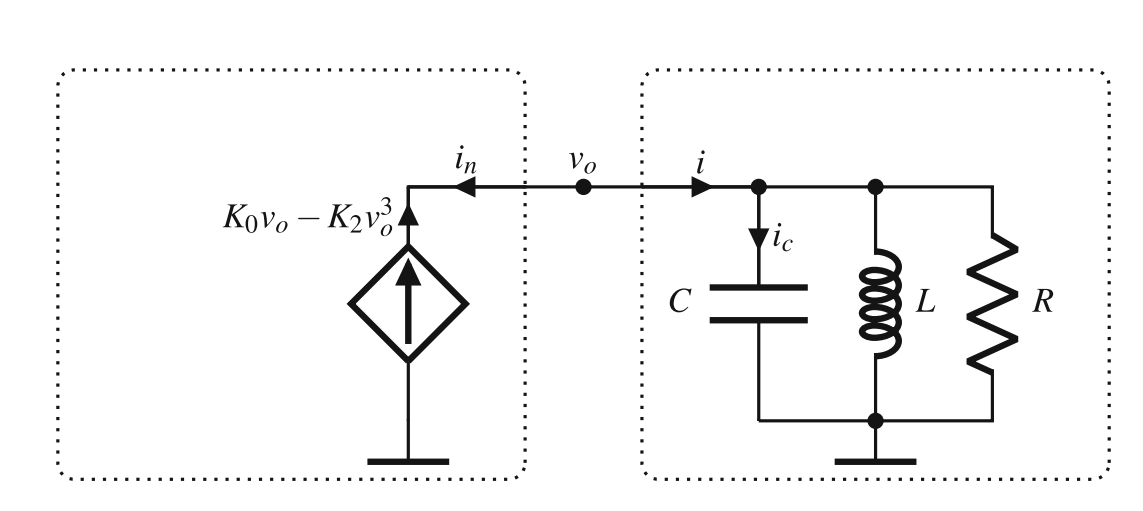
\includegraphics[width=0.8\linewidth]{VDPO.png}
    \caption{$\quad$范德波尔振子\textsuperscript{\cite{Casaleiro2019}}}
\end{figure}



范德波尔振子所满足的微分方程的通式为
\begin{equation}
    \frac{d^2 x}{dt^2}-\mu(1-x^2)\frac{dx}{dt}+x=0
\end{equation}
其中$x(t)$为位置坐标,$\mu$是表示非线性和阻尼强度的标量参数。

当$\mu=0$,即不存在阻尼函数时,方程变为
\begin{equation}
    \frac{d^2 x}{dt^2}+x=0
\end{equation}
此时为简谐振动的运动方程。

当$\mu>0$时,对于所有的初始条件,最终均会收敛为唯一的极限环。这个结论可以通过以下定理证明:

\begin{definition}
    对于系统
    $$x''+u(x)x'+v(x)=0$$
    若$f,g$为在$R$上连续的函数,且$f$为偶函数,$g$为奇函数,则该系统称为Liénard equation。
\end{definition}

\begin{theorem}[Levinson-Smith定理]
    对于Liénard equation,若其满足以下条件
    \begin{enumerate}[align=left]
        \item $u(x)$为连续偶函数,$v(x)$为连续奇函数;
        \item 若$x>0$,则$v(x)>0$;
        \item $\displaystyle\lim_{x \to \infty}\int_{0}^{x}v(x)=\infty$;
        \item $ {\exists}k>0$,使得:
        \begin{enumerate}[label={}]
            \item $0<x<k$时$U(x)<0$,
            \item $x>k$时$U(X)>0$,$U'(X) \geq 0$,
            \item $\displaystyle\lim_{x \to \infty}U(x)=\infty$。
        \end{enumerate}


    \end{enumerate}
    则系统满足:
    \begin{enumerate}[label={}]
        \item 存在唯一临界点(0,0);
        \item 存在唯一非零闭合轨迹$C$且为包含原点的稳定极限环;
        \item$\lim{t \to \infty}$时所有非零轨迹旋转逼近$C$。
    \end{enumerate}   
\end{theorem}
此时VDPO微分方程可以写成以下形式:
\begin{equation}
    \left \{
    \begin{aligned}
    &x''+u(x)x'+v(x)=0\\
    &u(x)=-\mu(1-x^2)\\
    &v(x)=x\\
    \end{aligned}
\right.
\end{equation}
可以看出这个微分方程满足Levinson-Smith定理,因此具有一个极限环。

接下来计算振动周期。范德波尔振子没有解析解\textsuperscript{\cite{https://doi.org/10.1002/zamm.200310040}}。对于$\mu \rightarrow 0$的情况,可以利用Poincaré–Lindstedt Method进行近似求解。
令$\tau=\omega t,\omega=1+\mu\omega_1+\mu^2\omega_2+O(\mu^3)$,代入
\begin{equation}
    \omega^2\ddot{x}-\omega\mu(1-x^2)\dot{x}+x=0
\end{equation}
得到
\begin{equation} 
    \left \{
    \begin{aligned}
    &\ddot{x_0}+x_0=0\\
    &\ddot{x_1}+x_1+2\omega_1\ddot{x_0}+(x_0^2-1)\dot{x_0}=0\\
    &\ddot{x_2}+x_2+(\omega_1^2+2\omega_2)\ddot{x_0}+2\omega_1\ddot{x_1}+2x_0x_1\dot{x_0}+\omega_1(x_0^2-1)\dot{x_0}+\dot{x_1}(x_0^2-1)=0\\
    \end{aligned}
    \right.
\end{equation}
对于第一个方程,一般解为$x_0=Acos(\tau+\phi)$,取$\phi=0$,然后带入第二个方程,得到
\begin{equation}
    \ddot{x_1}+x_1+(A-\frac{A^3}{4})\sin\tau-2\omega_1A\cos\tau-\frac{A^3}{4}\sin(3\tau)=0
\end{equation}
需要满足
\begin{equation} 
    \left \{
    \begin{aligned}
    &A=\frac{A^3}{4}\\
    &2\omega_1A=0
    \end{aligned}
    \right.
\end{equation}
即可得到$A=2,\omega_1=0$。
对于方程$\ddot{x_1}+x_1=2\sin(3\tau)$,其通解为
\begin{equation}
    x_1=B\cos(\tau+\phi)-\frac{1}{4}\sin(3\tau)
\end{equation}
而$x_1$与$x_0$无关,因此取$x_1=-\frac{1}{4}\sin(3\tau)$,可以得到$\omega_2=-\frac{1}{16}$。
于是可以得到$\omega$的近似值:
\begin{equation}
    \omega=1-\frac{1}{16}\mu^2+O(\mu^3)
\end{equation}
如果提高计算精度,可以得到
\begin{equation}
    \omega=1-\frac{1}{16}\mu^2+\frac{17}{3072}\mu^4+O(\mu^6)
\end{equation}
振动周期可以由以下公式计算:
\begin{equation}
    T=\frac{2\pi}{\omega}
\end{equation}
当$\mu$增大时,振动周期的近似计算结果为\textsuperscript{\cite{book}}
\begin{equation}
    T=(3-2\ln2)\mu
\end{equation}

在$\mu<0$时,范德波尔振子表现出与$\mu>0$不同的运动状态。将式(4)写成以下形式:

\begin{equation} 
    \left \{
    \begin{aligned}
    &\frac{dx}{dt}=v\\
    &\frac{dv}{dt}=\mu(1-x^2)v-x\\
    \end{aligned}
    \right.
\end{equation}
将系统的状态用向量$\vec{r}=(x,v)$进行描述,
可以看到当系统处于稳定状态时,即$\frac{d\vec{r}}{dt}=0$时,满足
\begin{equation} 
    \left \{
    \begin{aligned}
    &v=0\\
    &x=0\\
    \end{aligned}
    \right.
\end{equation}
即无论什么初始情况最终都会趋向静止。

\subsection{\zihao{5}数值计算}

对于范德波尔振子,可以使用Python的scipy库进行数值计算以及信号处理,得到其相空间图与周期。

首先,在$\mu=1$时,取初始条件(x,v)为(0,1)和(3,1)进行周期计算以及相空间图的绘制,图2即为得到的相空间图。此时在相空间图上,初始条件分别位于极限环的内部与外部。
根据上面的理论推导,可以知道其周期近似为
\begin{equation}
    T=\frac{2\pi}{\omega}=\frac{2\pi}{1-\frac{1}{16}\mu^2+\frac{17}{3072}\mu^4+O(\mu^6)}=6.6627
\end{equation}
数值计算的周期分别为$T=6.6653$与$T=6.6713$,与理论计算的结果吻合得很好。同时可以发现与初始条件无关,最终相空间图会收敛与同一个极限环上,

\begin{figure}
    \centering
    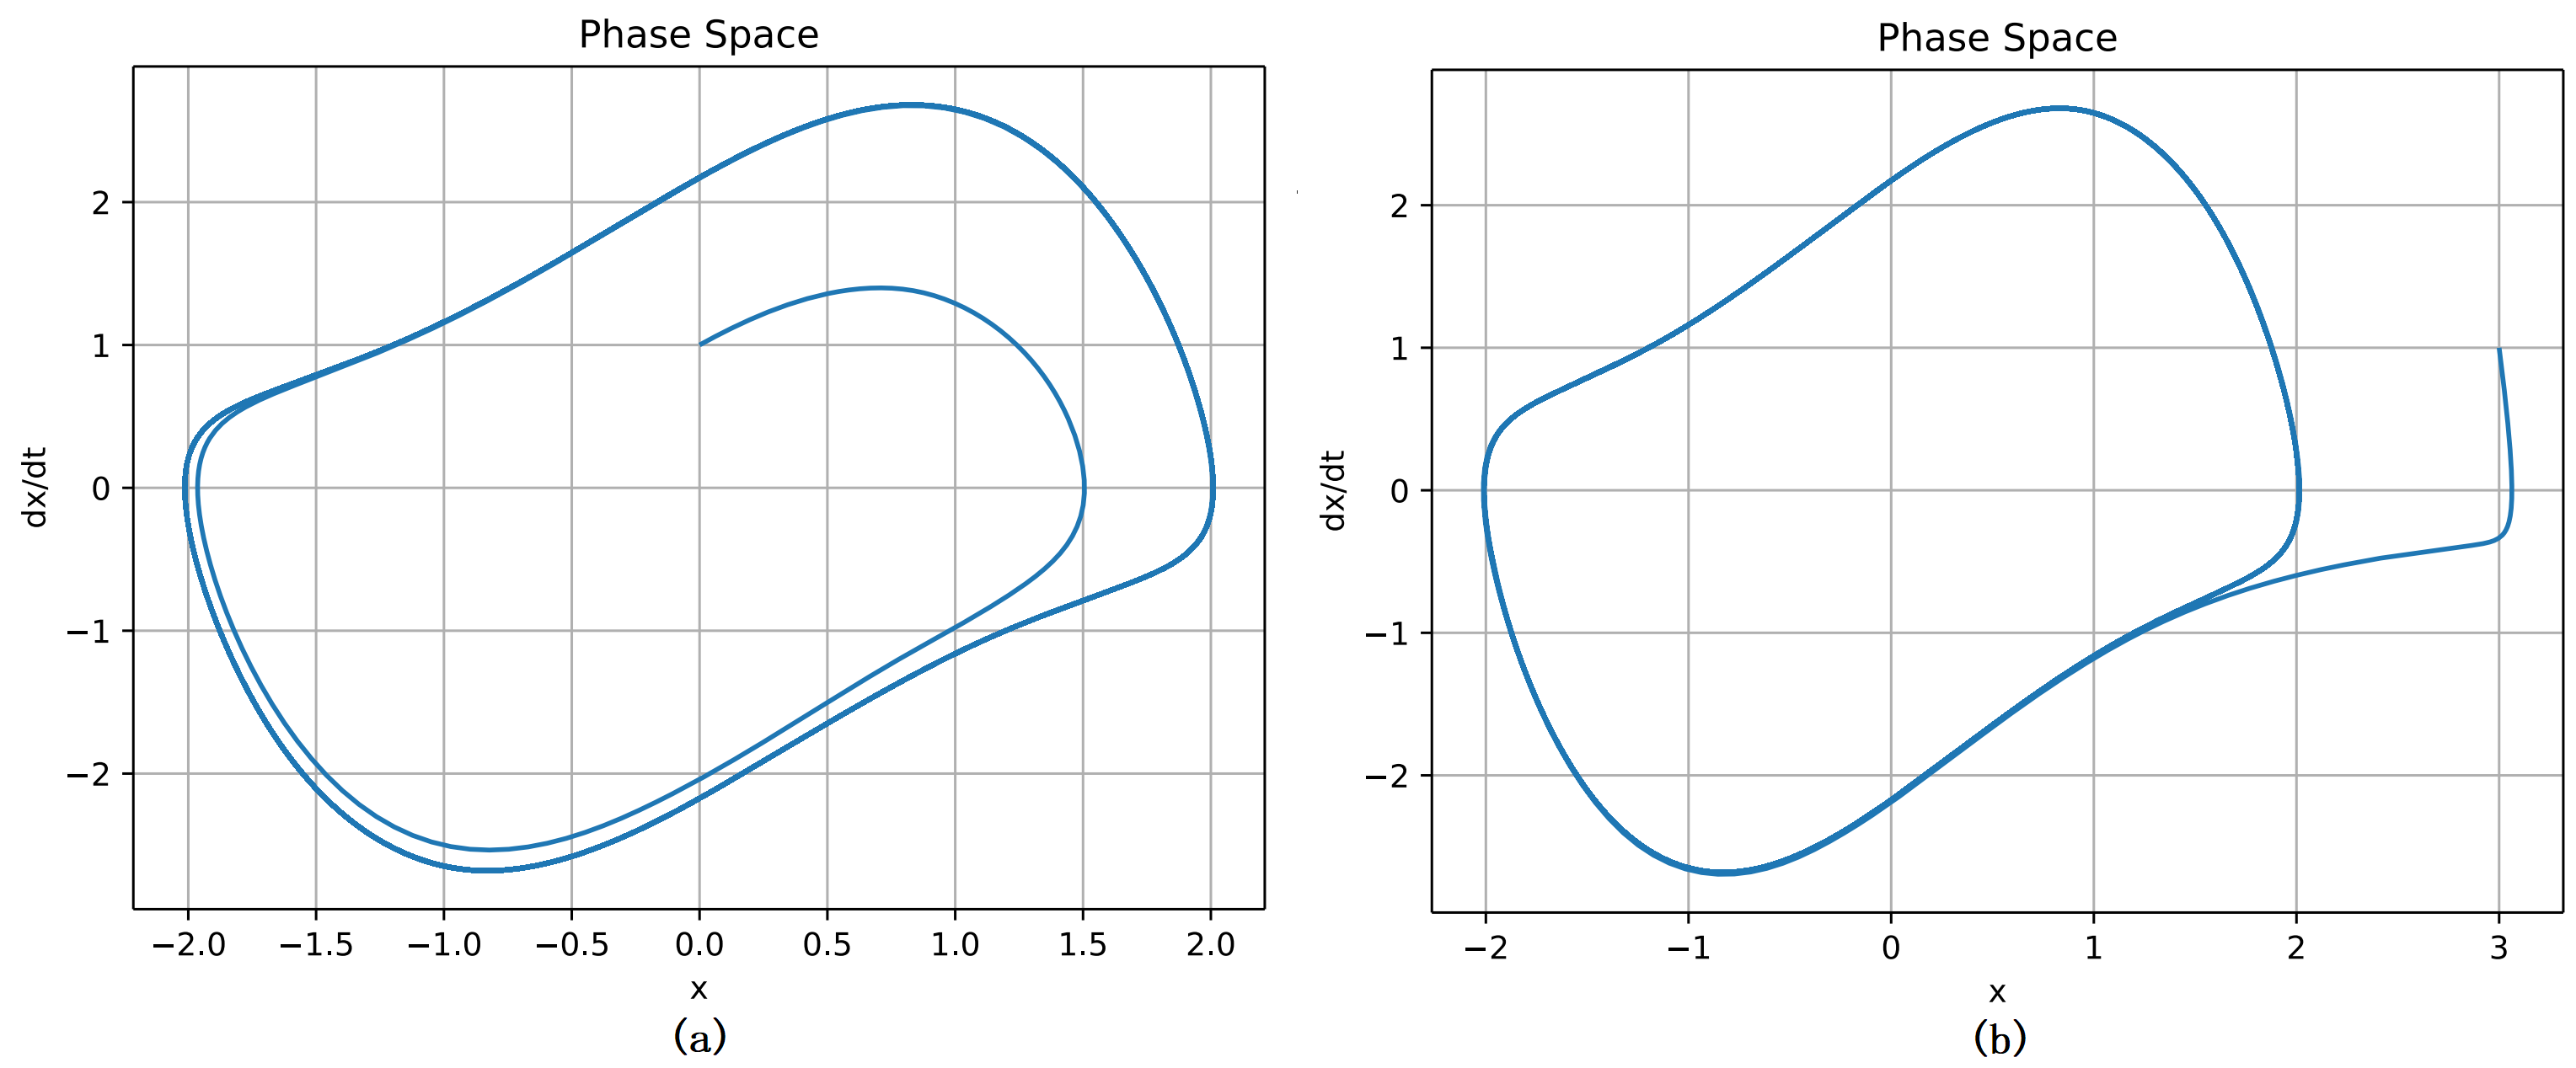
\includegraphics[width=0.8\linewidth]{1inout.png}
    \caption{$\quad$系统的初始值$(x,v)$分别为(a)$(0,1)$(b)$(3,1)$时的相空间图}
\end{figure}
  
接下来改变$\mu$的值,绘制在不同$\mu$值下的相空间图,得到图3。可以发现,随着$\mu$的增大,振动的振幅几乎不变,而速率的最大值越来越大,相空间图也越来越尖锐;
同时也可以得知范德波尔振子的振幅与$\mu$几乎无关。


\begin{figure}
    \centering
    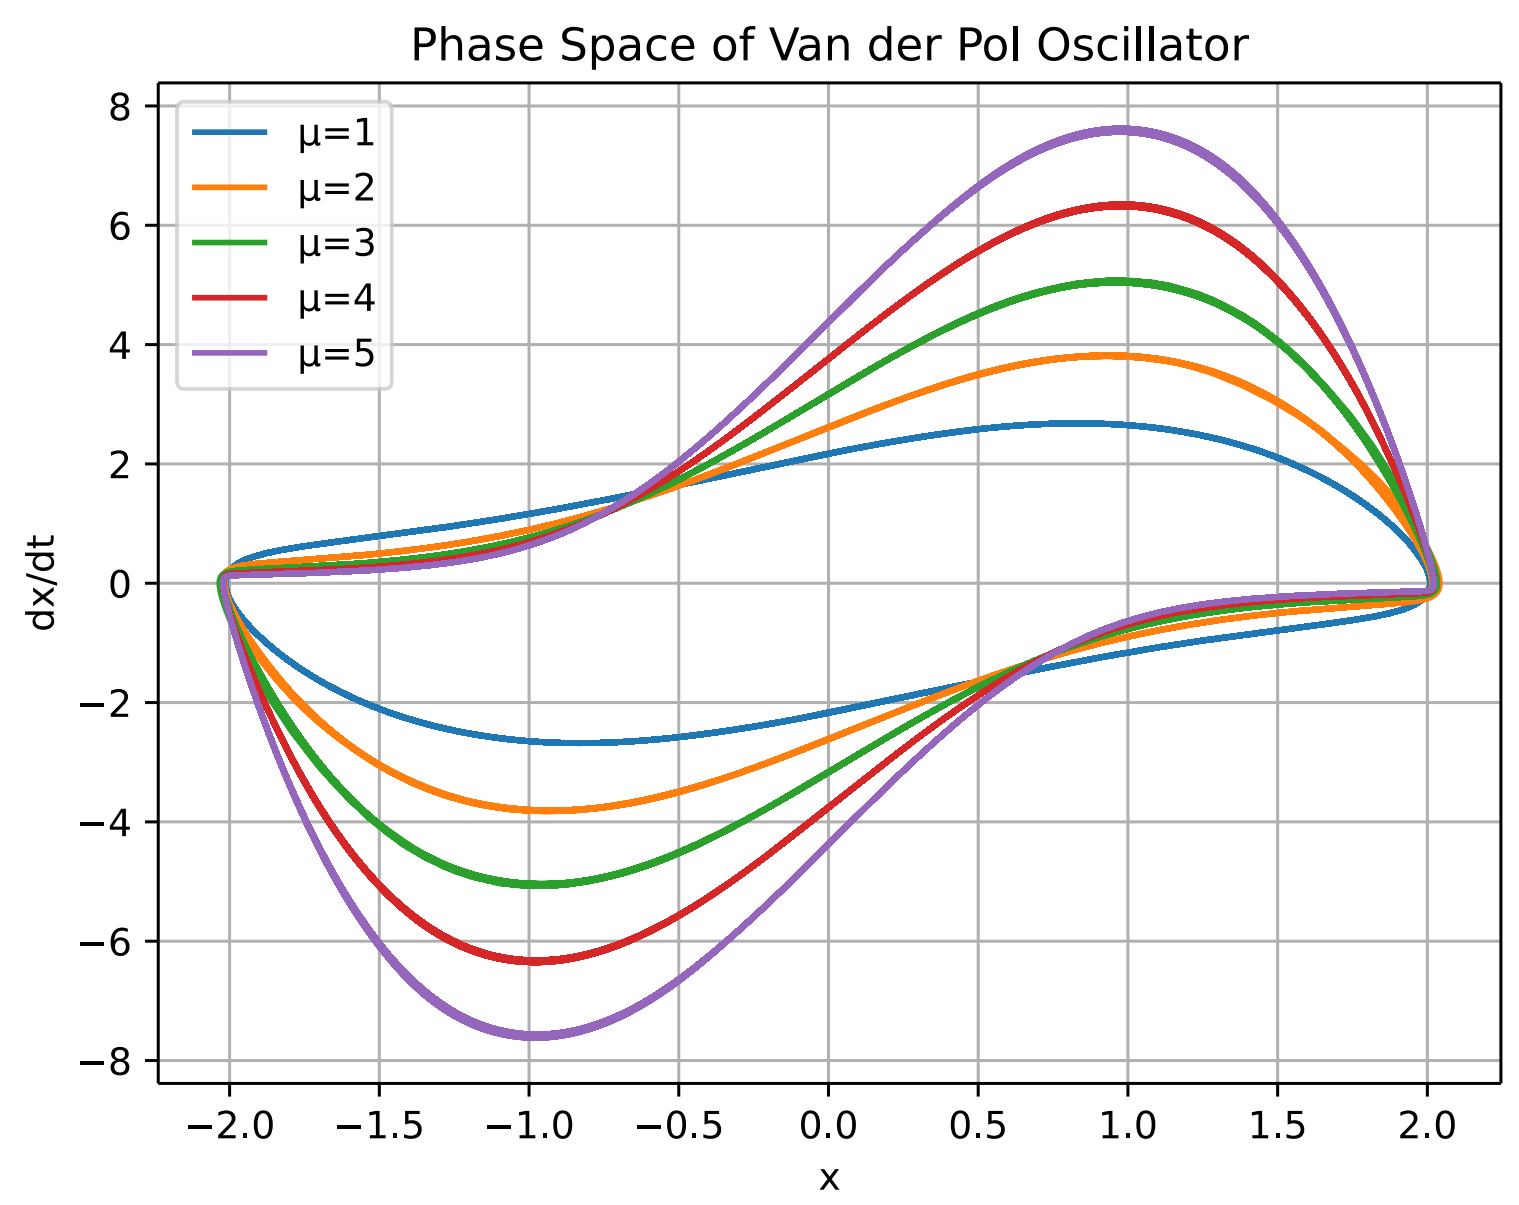
\includegraphics[width=0.4\linewidth]{1-5.png}
    \caption{$\quad$ 不同$\mu$值下的相空间中的极限环}
\end{figure}

\begin{figure}
    \centering
    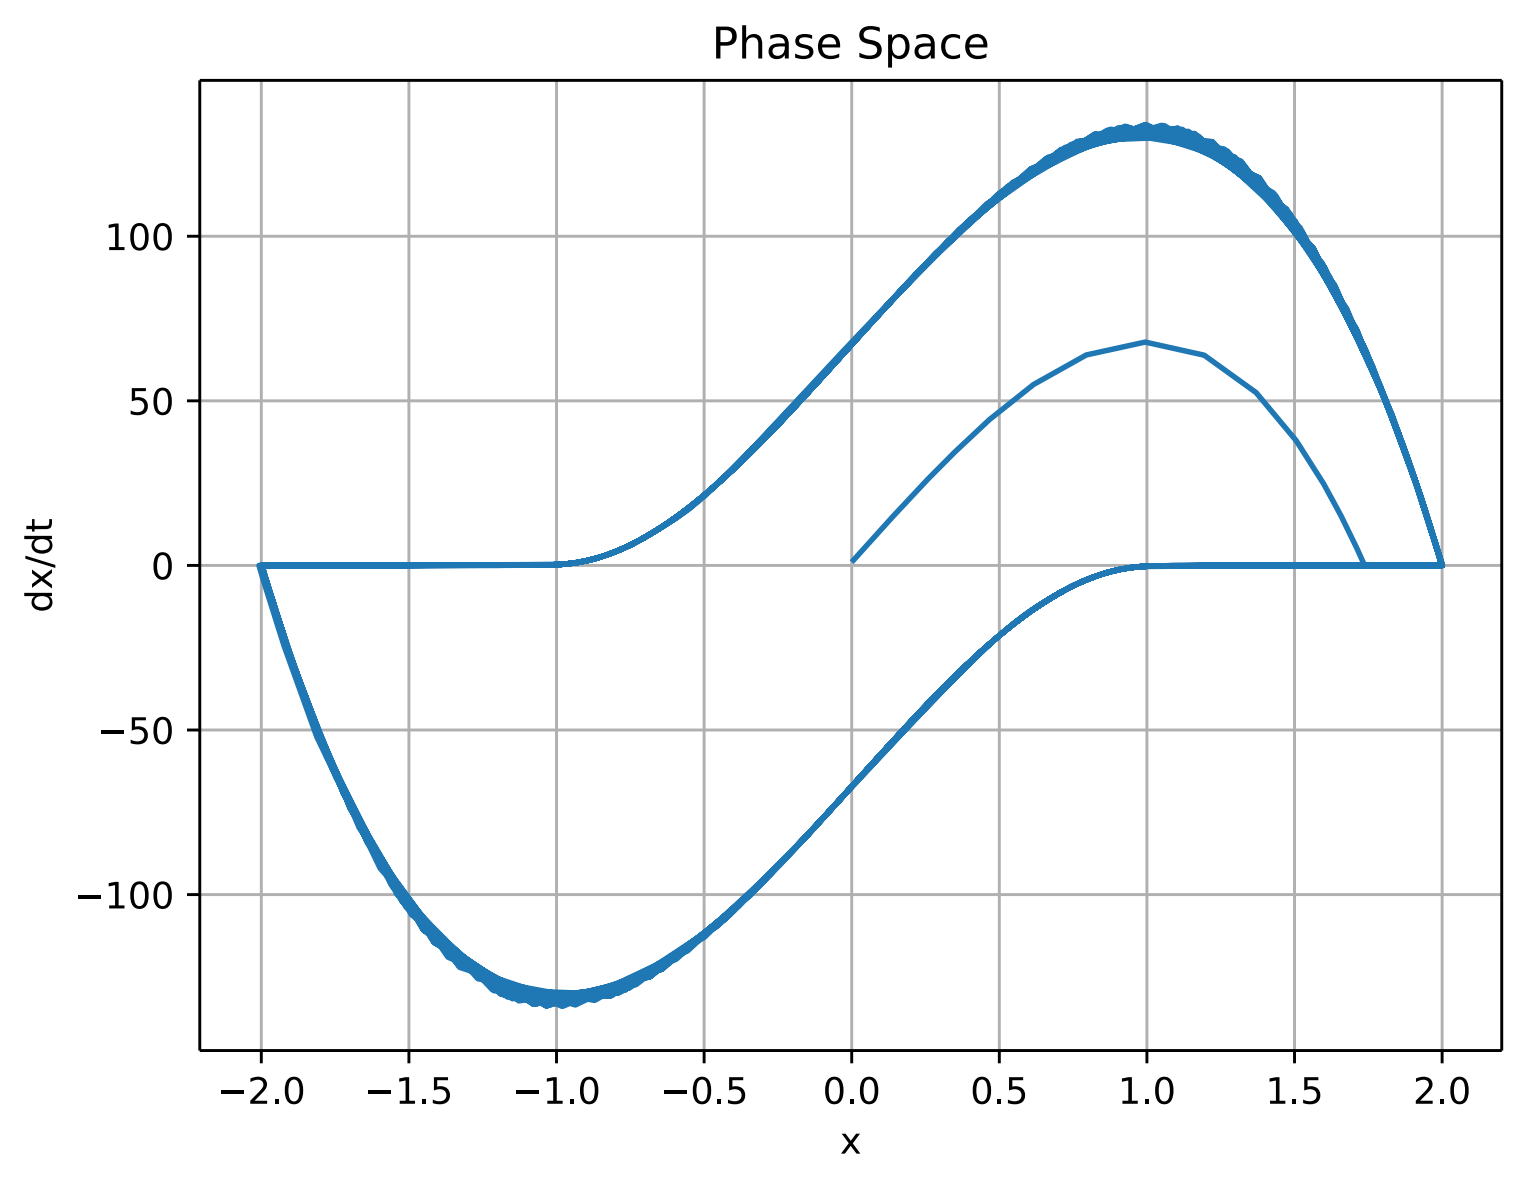
\includegraphics[width=0.5\linewidth]{100.png}
    \caption{$\quad$系统初始值为 $\mu=100, (x,v)=(0,1)$时的相空间图}
\end{figure}

改变$\mu$的值,计算$\mu=100$时振子的振动周期并绘制相空间图,如图4所示。此时理论计算得到的周期近似值为
\begin{equation}
    T=100(3-2\ln2)=161.3706
\end{equation}
数值计算得到的周期为$T=160.5240$,误差约为$0.52\%$,具有相当高的精度。

在$\mu<0$时同样可以得到其相空间图。取$\mu=-0.1, (x,v)=(1,1)$进行计算,可以得到图5所示的图象。
\begin{figure}
    \centering
    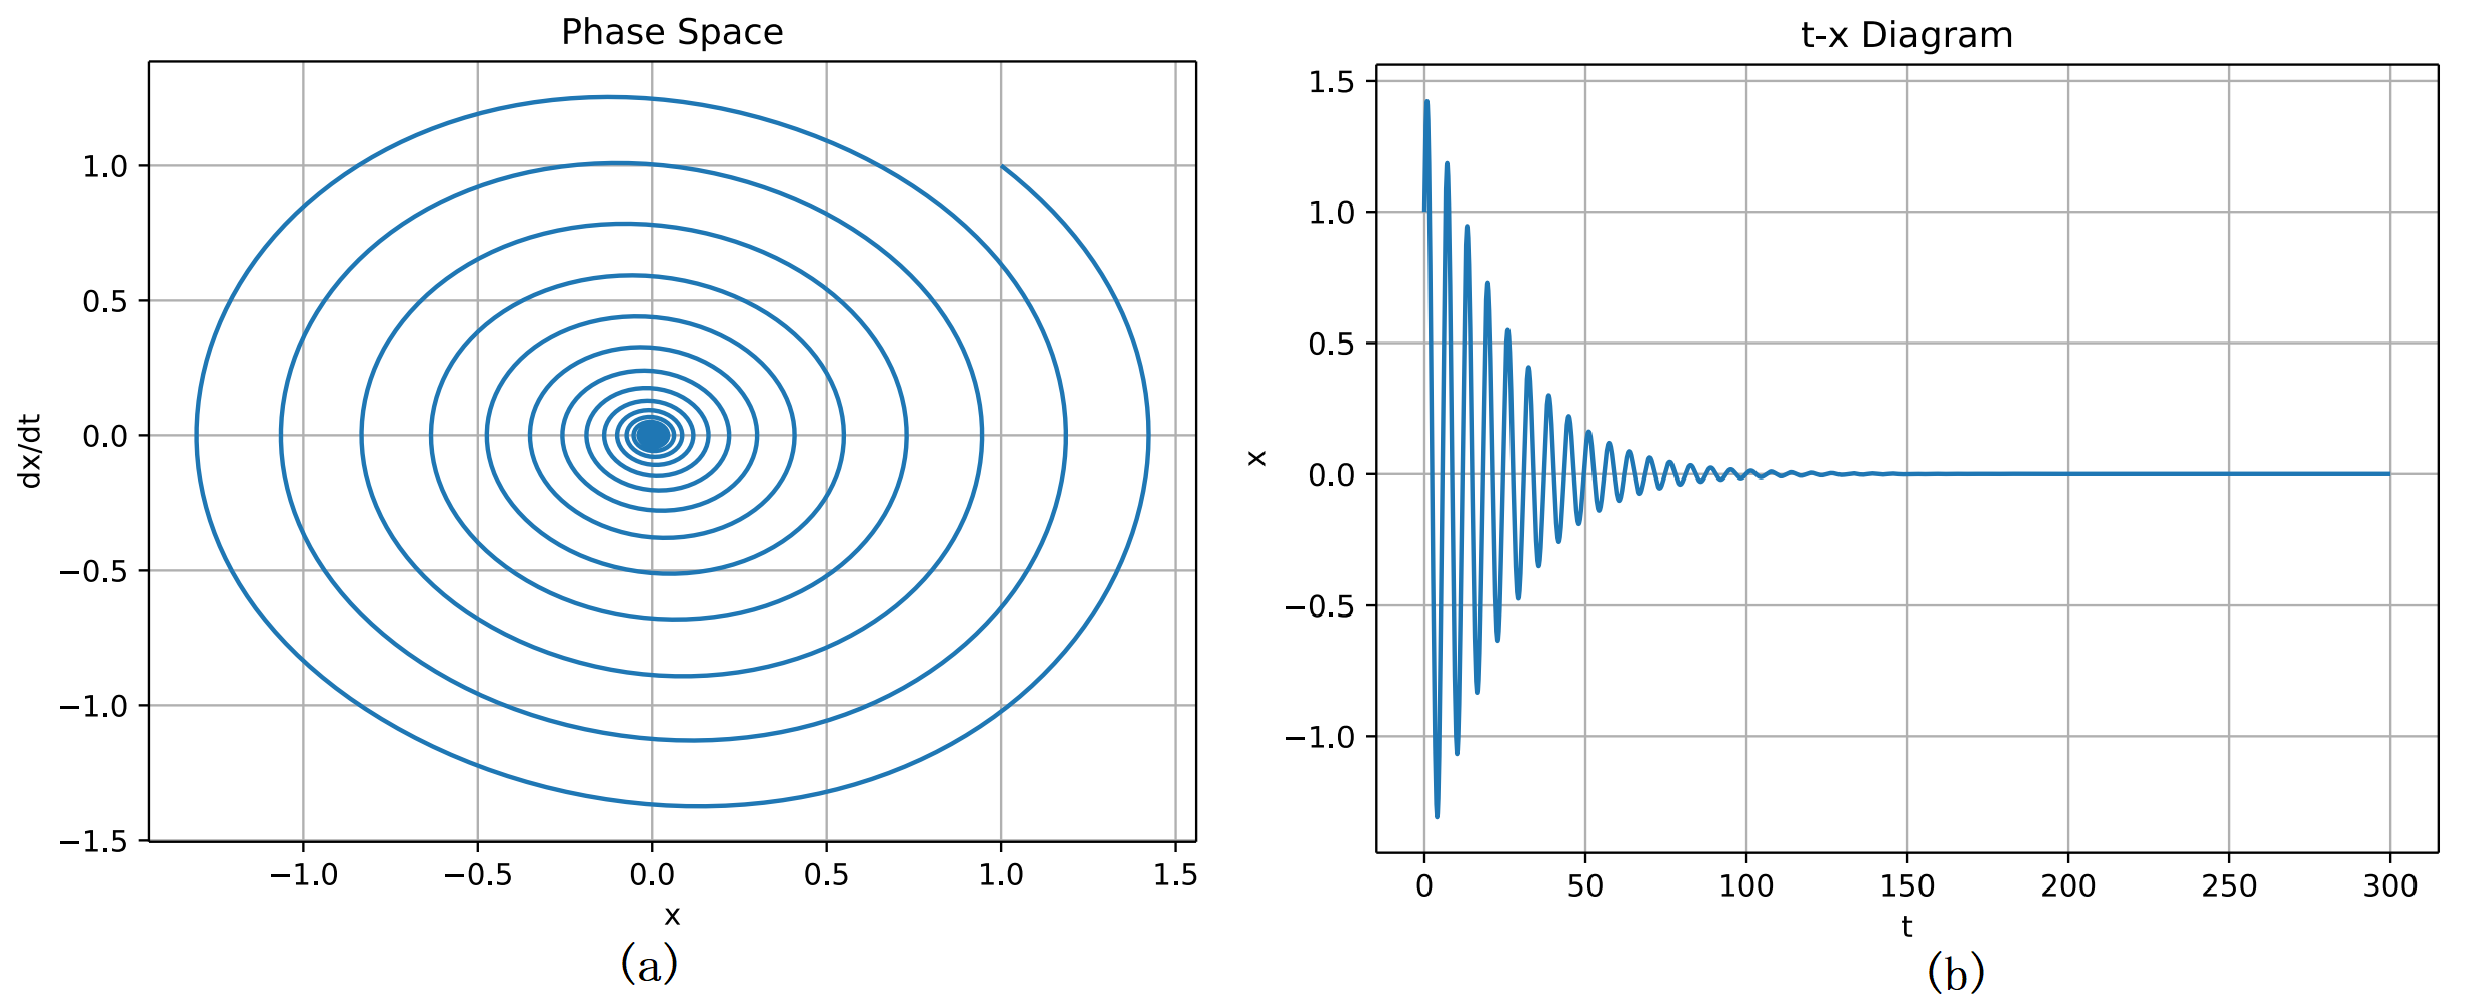
\includegraphics[width=0.8\linewidth]{xiaoyu.png}
    \caption{$\quad$系统初始值为 $\mu=-0.1, (x,v)=(1,1)$时的(a)相空间图,(b)时间-速度图像}
\end{figure}
可以发现此时系统最终会趋于静止,与上面得到的结论一致。

\section{\zihao{-4}结果与讨论}

对范德波尔振子的数值计算结果与理论结果进行分析,可以发现在不同$\mu$值的情况下两者均符合得较好:
在$\mu=1$的情况下周期误差不超过$0.13\%$,$\mu=100$时误差也仅有$0.52\%$,说明了采用的数值计算方法的有效性,并且验证了上面提出的理论模型。
同时对$\mu<0$的情况进行了定性分析,再次验证了理论部分的结论。

进一步分析两种计算方法之间的差异性与一致性可以发现,尽管理论计算和数值计算得到了相似的结果,但数值计算的精度收到了步长的限制,而理论计算的精度
受到级数展开项数的限制。两种方法各有优劣,理论方法的计算速度更快,而数值计算方法使用简单,并且对不同的初值具有更强的适应性。

由于篇幅限制,本文仅考虑了$\mu$对振动的影响,没有对其他因素(如无阻尼时的振动频率等)进行考虑,这可以成为其他研究的方向。

\newpage

\bibliographystyle{unsrt}
\bibliography{reference}

\newpage
\section*{\zihao{-4}附录}

本文中使用的代码如下:
\begin{lstlisting}[style = python]
    import numpy as np
    import matplotlib.pyplot as plt
    from scipy.integrate import solve_ivp
    from scipy.signal import find_peaks
    #输出高清矢量图
    %config InlineBackend.figure_format = 'svg'
    
    # 定义van der Pol oscillator的微分方程
    def vdp(t, y, u):
        x, dx_dt = y
        dy_dt = [dx_dt, u * (1 - x**2) * dx_dt - x]
        return dy_dt
    
    # 定义计算周期的函数
    def calculate_period(time, signal):
        peaks, _ = find_peaks(signal)
        periods = np.diff(time[peaks])
        avg_period = np.mean(periods)
        return avg_period
    
    # 相空间图绘制
    def plot_phase_space(x, dx_dt):
        plt.figure()
        plt.plot(x, dx_dt)
        plt.xlabel('x')
        plt.ylabel('dx/dt')
        plt.title('Phase Space')
        plt.grid(True)
        plt.show()
    
    # 相空间图绘制
    def plot_t_x(time, x):
        plt.figure()
        plt.plot(time, x)
        plt.xlabel('t')
        plt.ylabel('x')
        plt.title('t-x Diagram')
        plt.grid(True)
        plt.show()
    
    
    #定义解vdp函数并得到极限环
    def solvevdp(u, t_start, t_end, num_points, initial_conditions):
        #initial_conditions=[x(0), dx/dt(0)]
        x_list = []
        dx_dt_list = []
        solution = solve_ivp(lambda t, y: vdp(t, y, u),
                         [t_start, t_end],
                         initial_conditions,
                         t_eval=np.linspace(t_start, t_end, num_points))
        
        x = solution.y[0]
        dx_dt = solution.y[1]
        start_index = int(num_points * 0.2)  # 从轨迹的 20% 处开始
        x = x[start_index:]
        dx_dt = dx_dt[start_index:]
        x_list.append(x)
        dx_dt_list.append(dx_dt)
    
        return x_list, dx_dt_list
\end{lstlisting}

\begin{lstlisting}[style = python]
    #计算u = 1.0时的周期
    initial_conditions = [0, 1]  # x(0), dx/dt(0)
    u = 1.0
    t_start = 0.0
    t_end = 3000.0
    num_points = 100000

    solution = solve_ivp(lambda t, y: vdp(t, y, u),
                    [t_start, t_end],
                    initial_conditions,
                    t_eval=np.linspace(t_start, t_end, num_points))

    time = solution.t
    x = solution.y[0]
    dx_dt = solution.y[1]

    period = calculate_period(time, x)
    print("Van der Pol oscillator的周期为:", period)

    plot_phase_space(x, dx_dt)
\end{lstlisting}

\begin{lstlisting}[style = python]
    #计算u = 1.0时的周期,这次起始点在相空间外面
    initial_conditions = [3, 1]  # x(0), dx/dt(0)
    u = 1.0
    t_start = 0.0
    t_end = 3000.0
    num_points = 100000
    
    solution = solve_ivp(lambda t, y: vdp(t, y, u),
                        [t_start, t_end],
                        initial_conditions,
                        t_eval=np.linspace(t_start, t_end, num_points))
    
    time = solution.t
    x = solution.y[0]
    dx_dt = solution.y[1]
    
    period = calculate_period(time, x)
    print("Van der Pol oscillator的周期为:", period)
    
    plot_phase_space(x, dx_dt)
\end{lstlisting}

\begin{lstlisting}[style = python]
    # 绘制μ = 1 to 5的相空间图
    fig, ax = plt.subplots()
    
    for μ in range(1, 6):
        x, dx_dt = solvevdp(μ, 0, 3000, 100000, [1.0, 0.0])
        ax.plot(x[0], dx_dt[0], label=f'μ={μ}')
    
    ax.set_title('Phase Space of Van der Pol Oscillator')
    ax.set_xlabel('x')
    ax.set_ylabel('dx/dt')
    ax.legend()
    ax.grid(True)
    plt.show()
\end{lstlisting}

\begin{lstlisting}[style = python]
    #计算u = 100.0时的周期
    initial_conditions = [0, 1] 
    u = 100.0
    t_start = 0.0
    t_end = 3000.0
    num_points = 1000000
    
    solution = solve_ivp(lambda t, y: vdp(t, y, u),
                        [t_start, t_end],
                        initial_conditions,
                        t_eval=np.linspace(t_start, t_end, num_points))
    
    time = solution.t
    x = solution.y[0]
    dx_dt = solution.y[1]
    
    period = calculate_period(time, x)
    print("Van der Pol oscillator的周期为:", period)
    
    plot_phase_space(x, dx_dt)
\end{lstlisting}

\begin{lstlisting}[style = python]
    #绘制u<0时的相空间图与t-x图
    initial_conditions = [1 ,1]  # x(0), dx/dt(0)
    u = -0.1
    t_start = 0.0
    t_end = 300.0
    num_points = 1000000
    
    solution = solve_ivp(lambda t, y: vdp(t, y, u),
                        [t_start, t_end],
                        initial_conditions,
                        t_eval=np.linspace(t_start, t_end, num_points))
    
    time = solution.t
    x = solution.y[0]
    dx_dt = solution.y[1]
    
    
    
    plot_phase_space(x , dx_dt)
    plot_t_x(time , x)
\end{lstlisting}


\end{document}